% vim:ts=4:sw=4
% Copyright (c) 2014 Casper Ti. Vector
% Public domain.

\chapter{总结和展望}
\section{系统测试}
为了分析和评估本论文提出的基于人脸识别的匹配算法的有效性和可用性,我们使用了该算法编写的基于婚恋数据的匹配好友的应用进行了实验测试。本实验主要基于不同算法的匹配系统进行了分析评估。

本实验对于两个方面进行了分析和评估:
\begin{enumerate}
\item 数据库用户分析
\item 测试用户对于不同匹配算法的满意度
\end{enumerate}
\subsection{数据库用户分析}
通过数据库的采取的3000条数据进行分析,对于数据库的用户数据进行了统计。测试用户和数据库的用户的年龄分布如下图
\begin{figure}[h] 
\begin{minipage}[t]{0.65\linewidth}

\centering

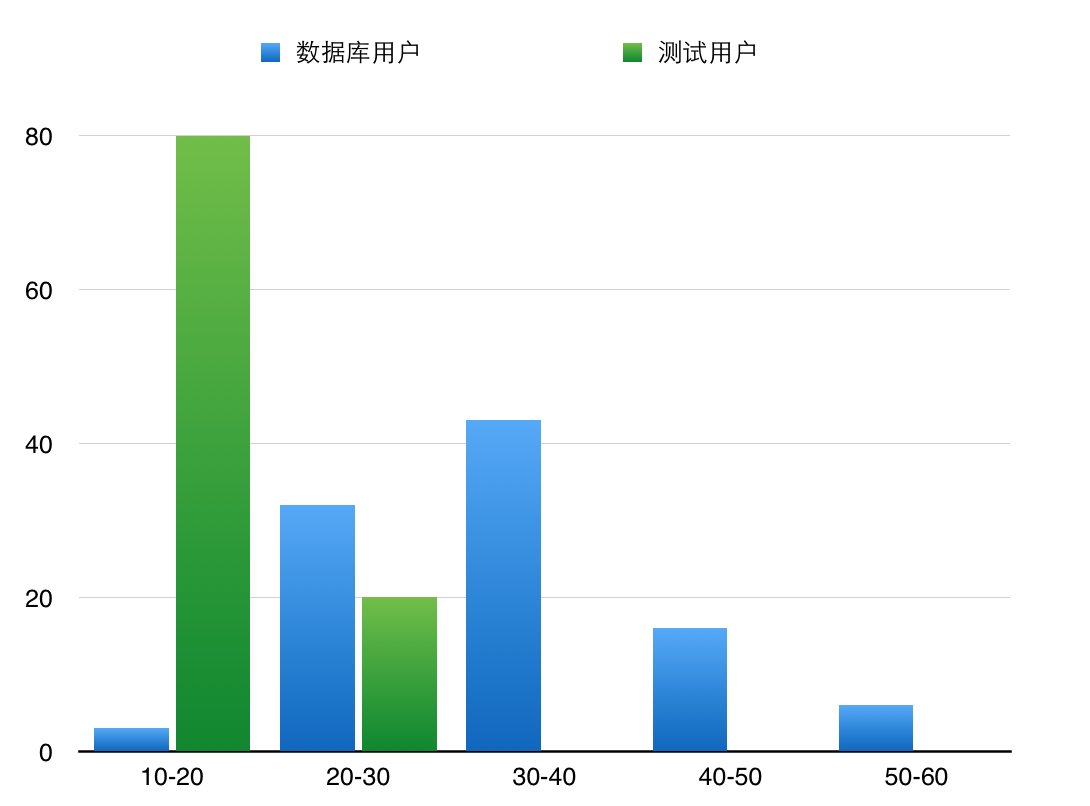
\includegraphics[width=\textwidth]{img/chap5/exp1.png}
\caption{年龄分布\label{instagram}}
\end{minipage}
\end{figure}

通过上表我们可以看出在数据库中的用户的年龄都偏大,超过半数的用户都超过了30岁,而测试用户却相反的半数以上都为30岁以下的青年人。带来这种差异的原因主要是数据库数据来源的特性,由于是婚恋网站,所以大多数的用户年龄都偏大,以及本文所邀请的用户的局限性主要限定在大学周围。由于年龄段的不同,用户有着不同的兴趣和审美观,而年龄差异过大的也并不适合称为一个社交圈子里的人。这种差异给匹配算法带来了一些不确定性。


但随着图片技术的发展(例如Microsoft的How old,如图5.2所示,可以大致检测出人的年龄),使得我	们可以在之后的工作中,为用户添加上这一特征值,从而进一步提供匹配算法的的准确性,降低这种差异给我们算法带来的不确定性。
\begin{figure}[h]
\begin{minipage}[t]{0.65\linewidth}
\centering
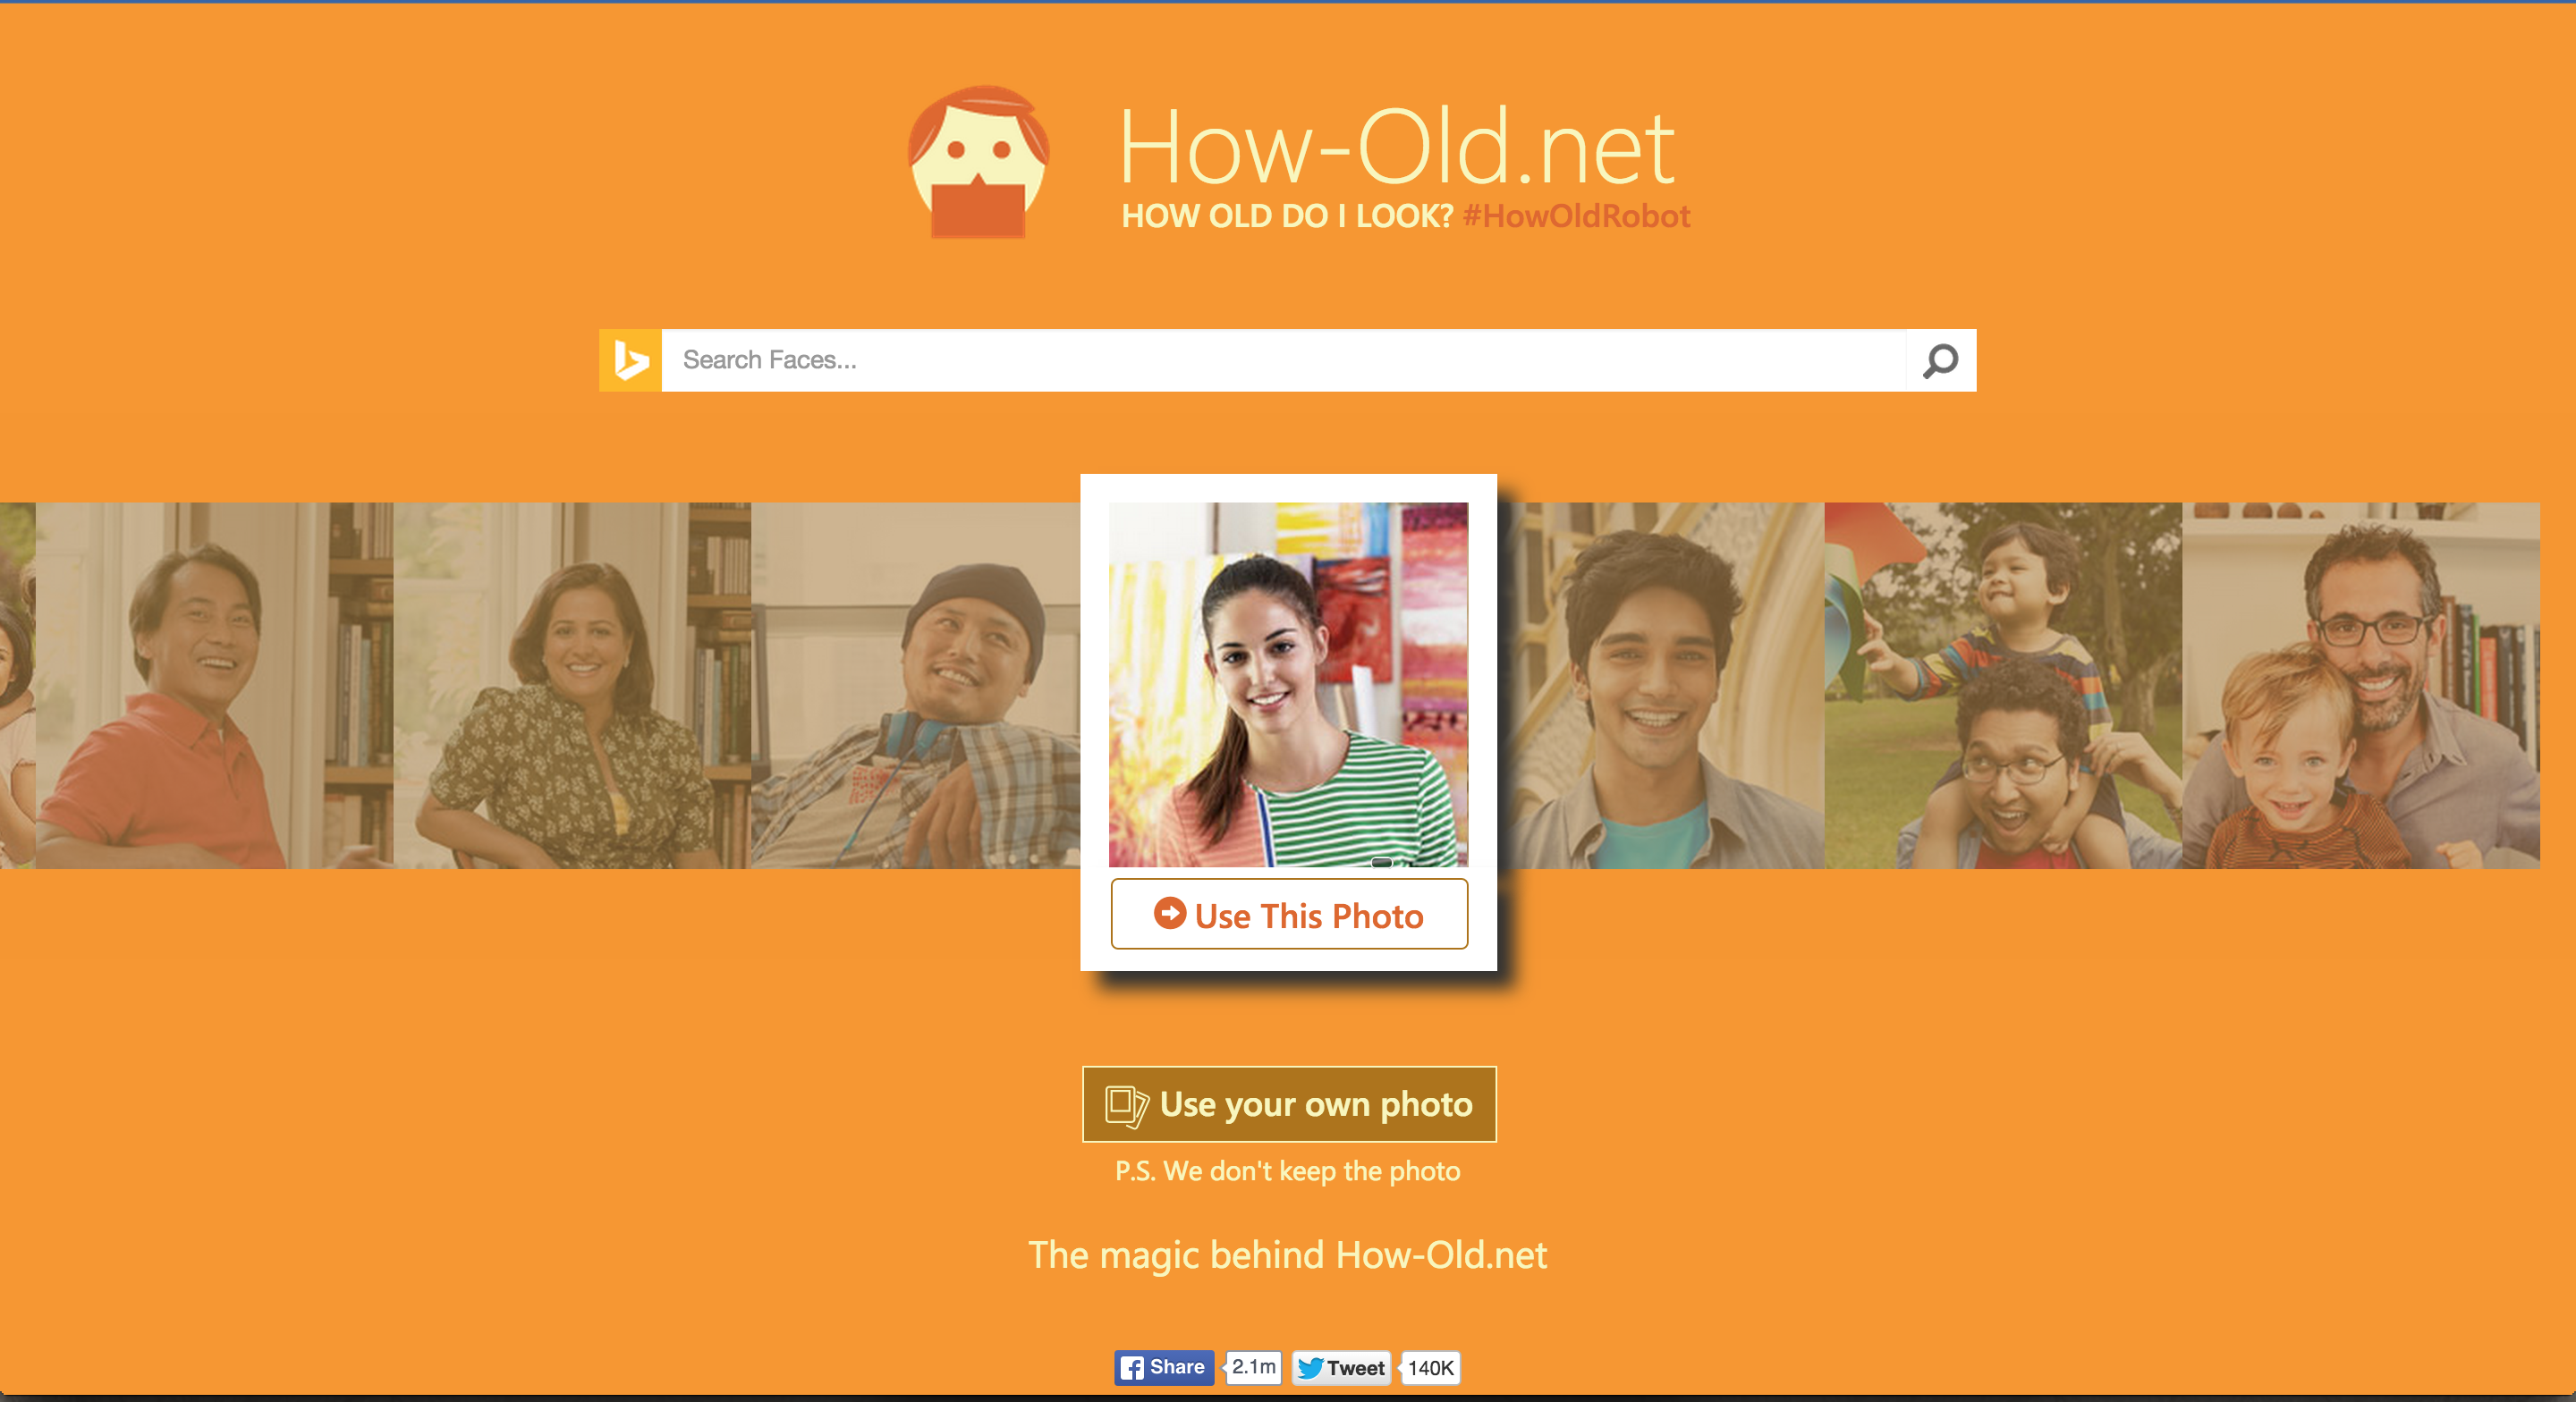
\includegraphics[width=\textwidth]{img/chap5/how_old.png}
\caption{How old from Microsoft\label{Face++API}}
\end{minipage}
\end{figure}

\subsection{实验结果}
总共20人参加了该实验的测试,该实验的满意度的分数为1-10分,测试用户对于一个测试算法给出的5个推荐好友进行评分,最后去一个平均值作为最终的检测结果。而对于不同的匹配算法的满意度的结果如下图。
\begin{figure}[h]
\begin{minipage}[t]{1\linewidth} 
\centering
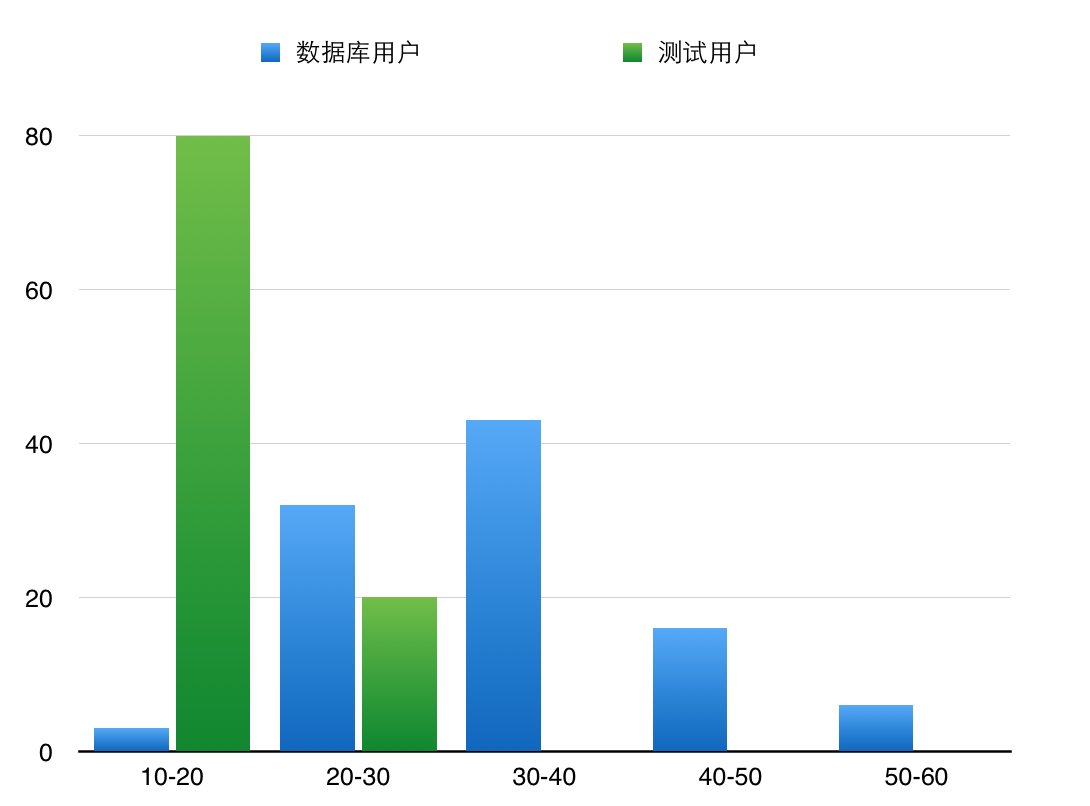
\includegraphics[width=\textwidth]{img/chap5/exp1.png}
\caption{满意度统计结果\label{instagram}}
\end{minipage}
\end{figure}
从表中可以看出由于加入了更多的一些特征到了匹配算法中,用户的满意度有了一定的提升。
% \section{匹配算法实验}
% \subsection{根据人脸相似度的匹配}
% \subsection{根据具体人脸特征的匹配}
% \subsection{根据具体信息的匹配算法}
% \subsection{机器学习算法}



